%\begin{figure}
%\centering
%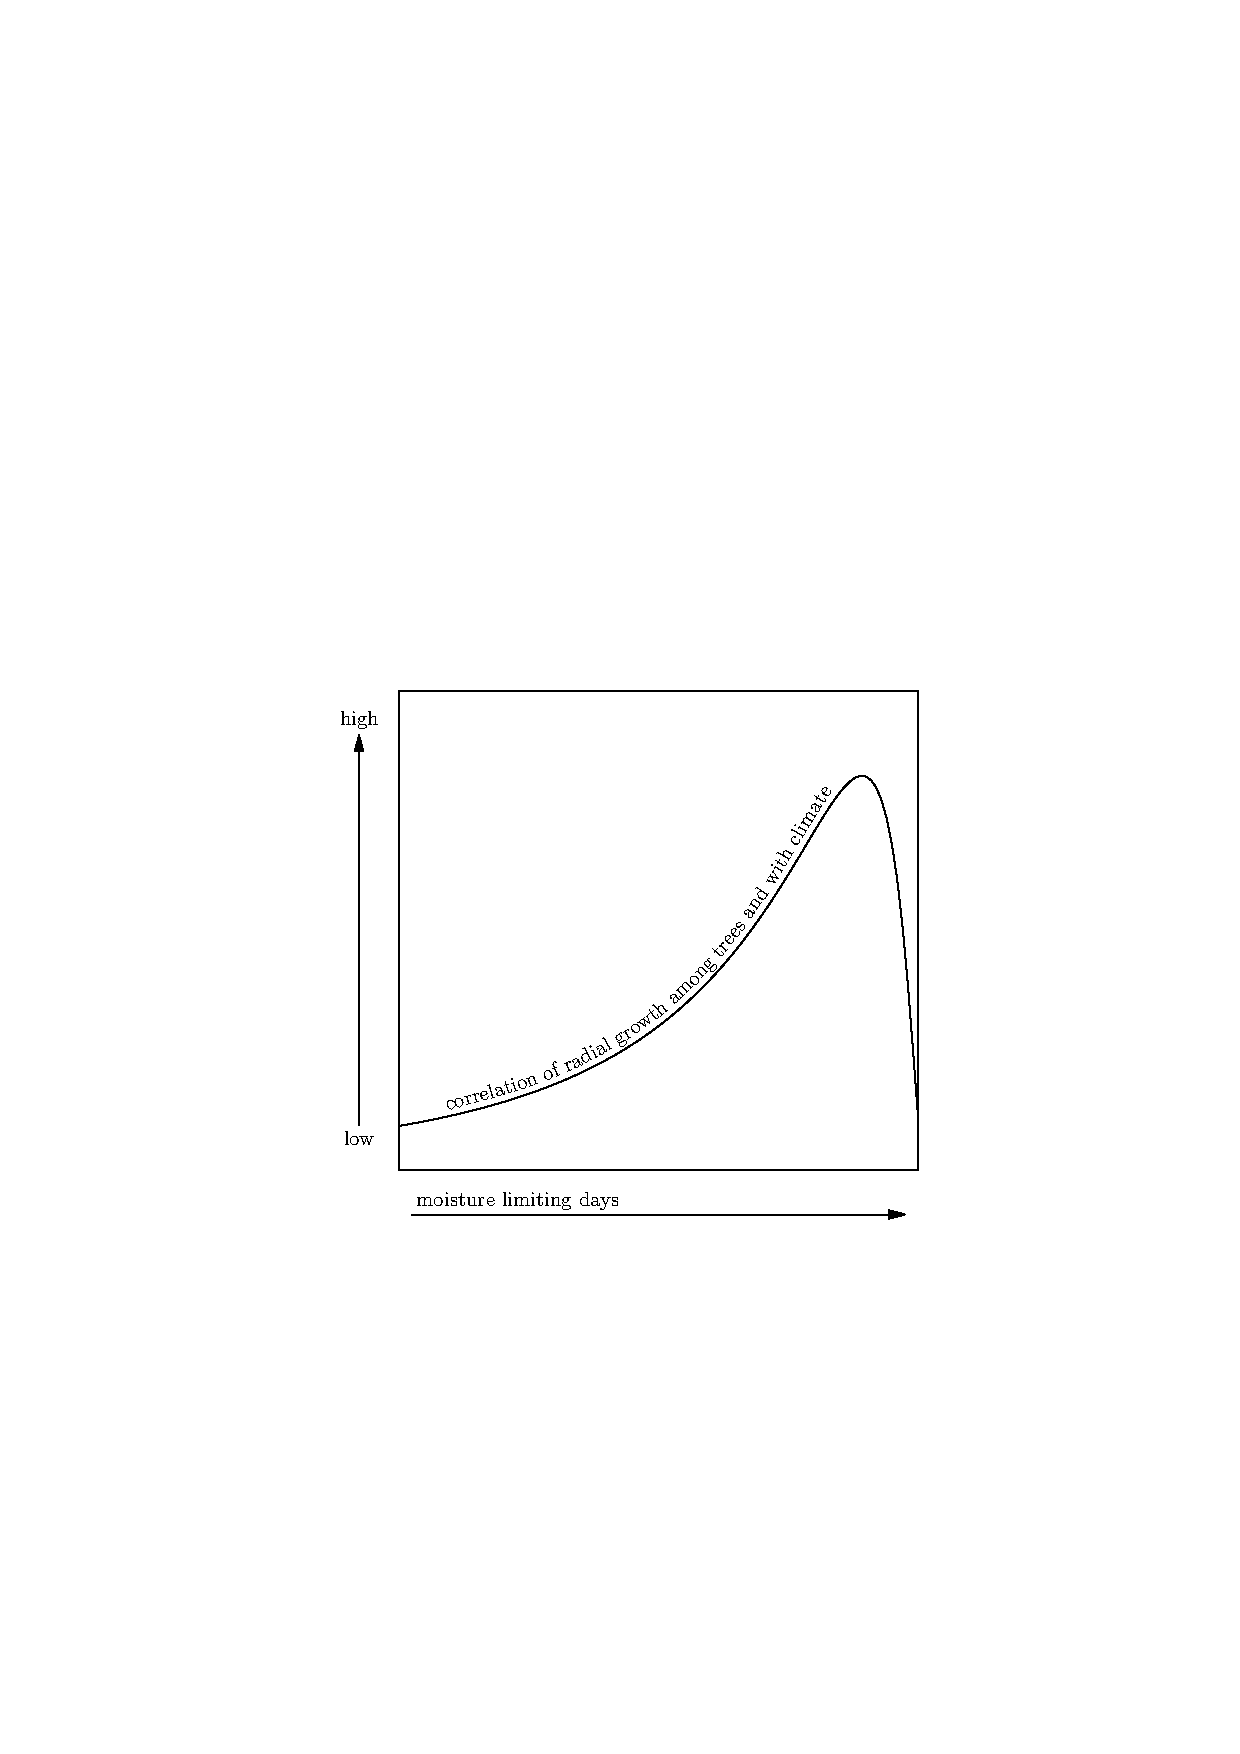
\includegraphics[width=6in]{figures/fritts.pdf}
%\caption{A simplified rendition of the diagram originally seen in \cite{fritts1976tree}.}
%\label{fig:fritts}
%\end{figure}

\begin{figure}
\centering
\includegraphics[width=5in]{figures/NewClimateNADEF.png}
\caption{Regional chronology sample locations.}
\label{fig:map}
\end{figure}

\begin{figure}
\centering
\includegraphics[width=5in]{figures/stacked_chrons.png}
\caption{Plots of the five chronologies used in the principal component analysis. The top panel shows the chronology built from the sample data at Brush Mountain (BM), while the others are the regional chronologies from Lynn Hollow (LH), watchdog Mountain (WD), Craig Creek (CC), and Otter Creek (OC).}
\label{fig:stackedChrons}
\end{figure}

\begin{figure}
\centering
\includegraphics[width=5in]{figures/scoresPlot.png}
\caption{Top: Scatter plot of the loadings for the five chronologies analyzed in the first PCA which covered the period 1845-1981. Bottom: Scatter plot of the loadings for the five chronologies analyzed in the second PCA which covered the period 1750-1981.}
\label{fig:scores}
\end{figure}

\begin{figure}
\centering
\includegraphics[width=5in]{figures/climCorr.png}
\caption{Top: Correlation between the growth proxies (BM or PC1) and the monthly precipitation from previous April (pA) through December (D) as well as for average May and June (aMJ). Middle: Correlation between the growth proxies (BM or PC1) and average PDSI from previous April (pA) through December (D) as well as for average June and July (aJJ). Bottom: Correlation between the growth proxies (BM or PC1) and average monthly temperature from previous April (pA) through December (D).}
\label{fig:climCorr}
\end{figure}

%\begin{figure}
%\centering
%\includegraphics[width=6in]{figures/climCorrTemp.pdf}
%\caption{Correlation between the growth proxies (BM or PC1) and average monthly temperature from previous April (pA) through December (D).}
%\label{fig:tempBarCorr}
%\end{figure}

%\begin{figure}
%\centering
%\includegraphics[width=6in]{figures/climCorrPdsi.pdf}
%\caption{Correlation between the growth proxies (BM or PC1) and average PDSI from previous April (pA) through December (D) as well as for averaged June and July (aJJ).}
%\label{fig:pdsiBarCorr}
%\end{figure}

\begin{figure}
\centering
\includegraphics[width=5in]{figures/corrMapPrecipMJ_bw_annot.png}
\caption{Correlation map showing the correlation between the first principal component and averaged May-June precipitation. Stars indicate the locations of the sites where the tree-rings used to develop the contributing chronologies were sampled.}
\label{fig:precipCorrMap}
\end{figure}

%\begin{figure}
%\centering
%\includegraphics[width=5in, angle=-90]{figures/corrMapPdsiJJ.pdf}
%\caption{Correlation map.}
%\label{fig:pdsiCorrMap}
%\end{figure}
%
%\begin{figure}
%\centering
%\includegraphics[width=5in, angle=-90]{figures/corrMapTempSept.pdf}
%\caption{Correlation map showing the correlation between the first principal component and September temperature.}
%\label{fig:tempCorrMap}
%\end{figure}

\begin{figure}
\centering
\includegraphics[width=5in]{figures/precipRunningCorr.png}
\caption{A 31-year windowed correlation plot showing the correlations between each growth proxy (chronologies and first principal component) and mjPR. Correlation points are plotted above the window centers.}
\label{fig:precipRunningCorr}
\end{figure}

\begin{figure}
\centering
\includegraphics[width=5in]{figures/recon.png}
\caption{Average May-June precipitation (mjPR) reconstruction (grey curve), smoothed estimate showing decadal-scale variable (black curve), and the reconstruction 95\% credible interval (shaded grey region).}
\label{fig:precipRecon}
\end{figure}

\begin{figure}
\centering
\includegraphics[width=5in]{figures/spectralRecon.png}
\caption{Periodogram showing periodicity of high amplitude at approximately 11, 17, and 24 years.}
\label{fig:spectral}
\end{figure}

\begin{figure}
\centering
\includegraphics[width=5in]{figures/reconsStacked.png}
\caption{Time series plots showing annual- and decadal-scale variability for the mjPR and six compared moisture reconstructions for the period 933-2008.}
\label{fig:allRecons}
\end{figure}

\begin{figure}
\centering
\includegraphics[width=5in]{figures/reconsStackedZoom.png}
\caption{Time series plots showing annual- and decadal-scale variability for the mjPR and six compared moisture reconstructions for the period 1745-1985.}
\label{fig:allReconsZoom}
\end{figure}


\begin{figure}
\centering
\includegraphics[width=5in]{figures/reconCompare.png}
\caption{Both the mjPR reconstruction and the Cook PDSI reconstruction are standardized and plotted against time to highlight both the similarities and the differences. Particularly notable differences include the year 1774, and the interval 1855-1863.}
\label{fig:reconCompare}
\end{figure}

\begin{figure}
\centering
\includegraphics[width=5in]{figures/wetdry.png}
\caption{The mjPR reconstruction (top panel) and the mjPR instrumental record (bottom panel). Lines show the best-fit regression line through the time series data to indicate any dominant trends. Areas falling above the best-fit lines and the time series data are shaded grey to indicate periods of higher precipitation. Note the correspondence of wetter and drier years between the top and bottom panels.}
\label{fig:wetdry}
\end{figure}

\begin{figure}
\centering
\includegraphics[width=5in]{figures/reconRunningCorr.png}
\caption{A 31 year windowed correlation plot between the mjPR and Cook PDSI reconstructions shows the discrepancy during the 1855-1863 interval. In the top panel correlation values are plotted about window centers, while the bottom panel shows the corresponding p-value (black) as well as the line of significance (dashed).}
\label{fig:reconRunningCorr}
\end{figure}

\begin{figure}
\centering
\includegraphics[width=5in]{figures/cookPdsiRunningCorr.png}
\caption{A 31 year windowed correlation plot between each of the chronologies and the Cook PDSI reconstruction. Note the interval of abrupt poor correlation during the years 1855-1863.}
\label{fig:cookRunningPdsiCorr}
\end{figure}

